\documentclass[aspectratio=169,12pt]{beamer}
\usepackage[T1]{fontenc}
\usepackage[utf8]{inputenc}
\usepackage{lmodern}
\usepackage[spanish]{babel}
\usepackage{graphicx}
\usepackage{amssymb}
\usepackage{tikz}
\usetikzlibrary{positioning,arrows.meta,calc}

% Paleta neutra: gris oscuro y azul petróleo
\definecolor{gris}{HTML}{2F3A40}
\definecolor{grisclaro}{HTML}{9AA5AB}
\definecolor{petroleo}{HTML}{1F6672}
\definecolor{fondo}{HTML}{EEF2F3}

\usetheme{default}
\setbeamertemplate{navigation symbols}{}
\setbeamercolor{normal text}{fg=gris}
\setbeamercolor{frametitle}{fg=petroleo}
\setbeamercolor{title}{fg=petroleo}
\setbeamercolor{structure}{fg=petroleo}
\setbeamerfont{frametitle}{series=\bfseries,size=\LARGE}
\setbeamertemplate{frametitle}{\vspace*{0.6em}\insertframetitle\par\vspace{-0.2em}{\color{petroleo}\rule{3cm}{1.2pt}}}
\setbeamertemplate{footline}{\hfill{\color{grisclaro}\scriptsize\insertframenumber}\hspace*{1.2em}\vspace*{0.8em}}

\newcommand{\frente}[2]{%
    \begin{beamercolorbox}[wd=\linewidth,sep=5pt,rounded=false]{bloque}
      {\color{petroleo}\bfseries #1}\par\vspace{0.2em}\small #2
    \end{beamercolorbox}}

\newcommand{\punto}{{\color{petroleo}$\blacktriangleright$}\ }
\newcommand{\fuente}[1]{\par\vfill{\color{grisclaro}\scriptsize #1}}

\title{Contabilidad de la muerte: por qué una reforma fiscal pequeña no basta}

\begin{document}

% ---------- 1. Portada ----------
\begin{frame}[plain]
  \vspace*{1.2em}
  {\color{petroleo}\bfseries\fontsize{24}{29}\selectfont Contabilidad de la muerte:\\[0.2em]
  por qué una reforma fiscal pequeña no basta\par}
  \vspace{0.4em}{\color{petroleo}\rule{4cm}{1.5pt}}\par
  \vspace{1.2em}
  {\large\bfseries Héctor Juan Villarreal Páez\par}
  {\normalsize Escuela de Gobierno y Transformación Pública, Tecnológico de Monterrey\par}
  \vspace{1.4em}
  {\small Congreso SobreMéxico 2026\\
  Mesa de discusión 1 · Repensando las finanzas públicas: una perspectiva de mediano y largo plazo\\
  Organiza: Departamento de Economía, Universidad Iberoamericana\\[0.5em]
  Auditorio Ernesto Meneses, Universidad Iberoamericana · 22 de octubre de 2026\par}
\end{frame}

% ---------- 2. Punto de partida ----------
\begin{frame}{El gasto ya supera al ingreso, y la diferencia se financia con deuda}
  \begin{columns}[c]
    \begin{column}{0.58\textwidth}
      \centering
      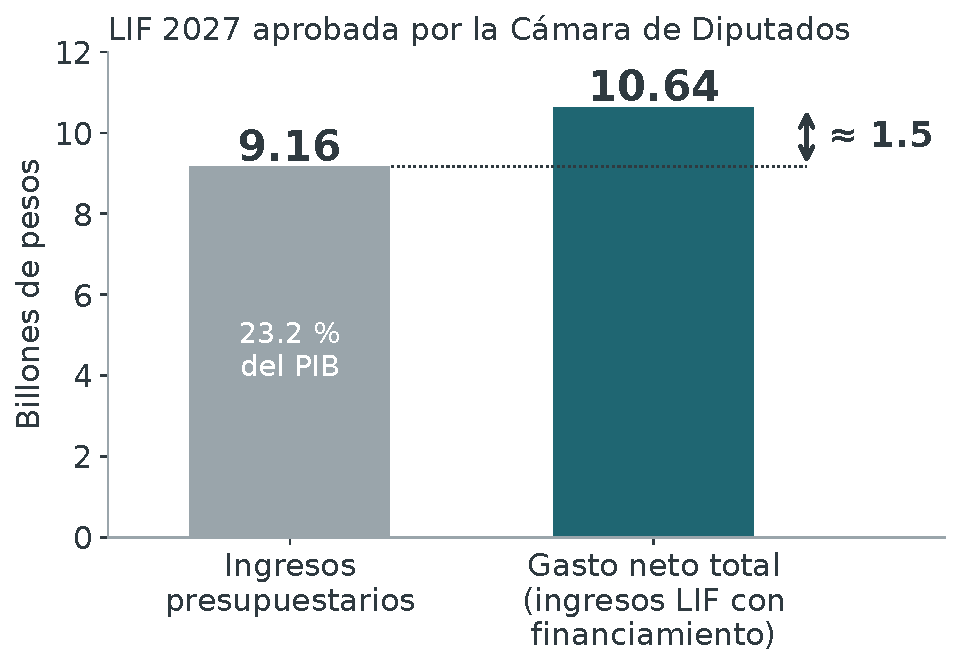
\includegraphics[height=0.46\textheight]{fig/l2_ingresos_gasto_lif2027.pdf}\par
      \vspace{0.1em}{\footnotesize RFSP 3.9\,\% del PIB · Deuda amplia 55\,\% del PIB\par}
    \end{column}
    \begin{column}{0.38\textwidth}
      \Large En 2027 el gasto supera a los ingresos presupuestarios por
      {\color{petroleo}\bfseries $\approx$\,1.5 billones} de pesos.
    \end{column}
  \end{columns}
  \fuente{LIF 2027 aprobada por la Cámara de Diputados; fuente: dictamen LIF 2027, Cámara de Diputados. RFSP y su saldo histórico: Paquete Económico 2027; fuente: SHCP, CGPE 2027.
  Razones calculadas con el PIB de SHCP; con un PIB más conservador serían algo mayores.}
\end{frame}

% ---------- 3. Contabilidad de la muerte ----------
\begin{frame}{De cada peso, casi todo ya tiene dueño}
  \centering
  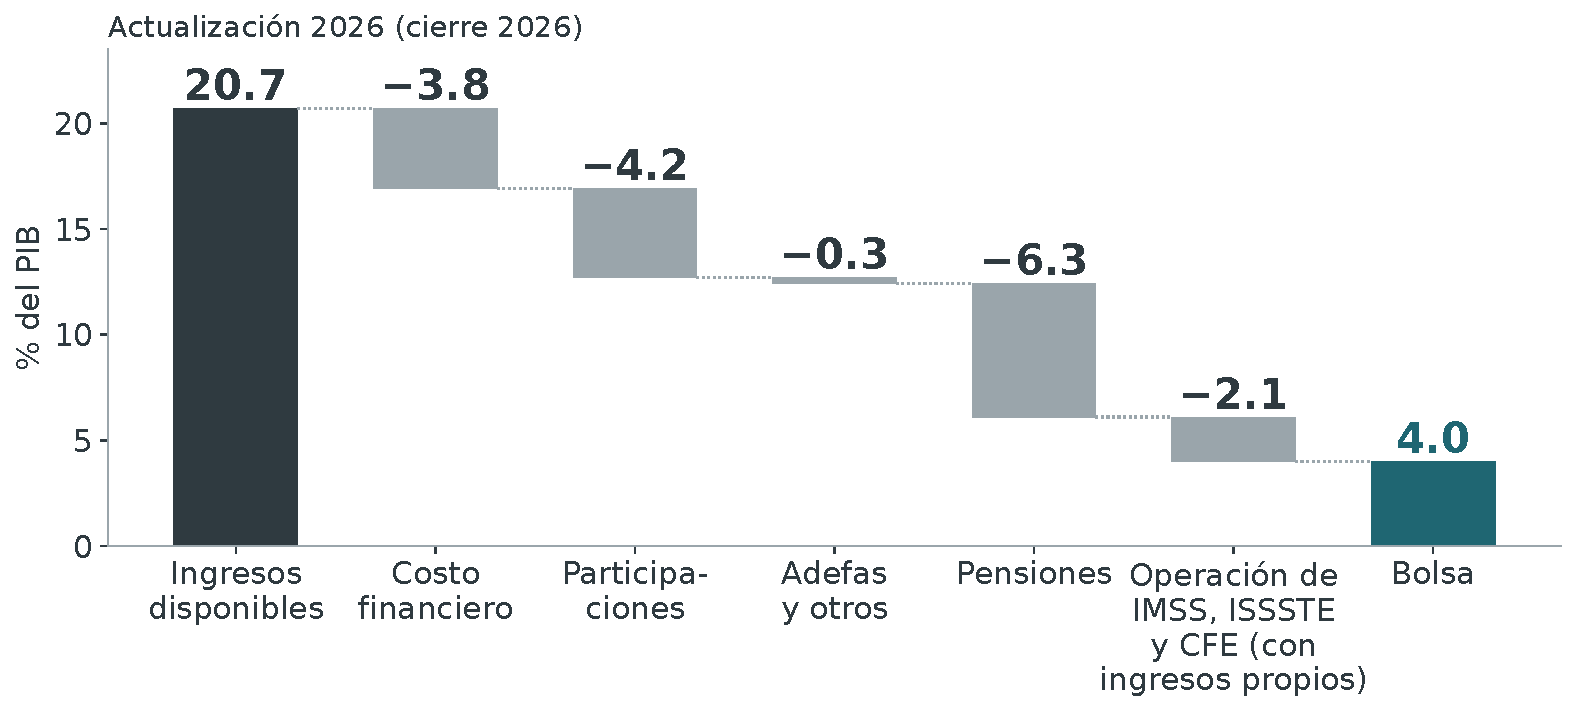
\includegraphics[width=0.80\textwidth]{fig/l3_cascada_2026.pdf}\par
  \vspace{0.1em}
  {\small Sin petroleros: transferencias del FMP (0.7) y apoyos a Pemex (0.7) se compensan.\par}
  \fuente{Supuestos generosos con la SHCP (PIB nominal 2026 de 36,500 mmdp); la bolsa real probablemente es menor. Actualización 2026.
  Fuente: elaboración propia con datos de SHCP (enero--julio 2026, cifras anuales estimadas).}
\end{frame}

% ---------- 4. Todo compite por la Bolsa ----------
\begin{frame}{Todo compite por la Bolsa}
  \begin{columns}[c]
    \begin{column}{0.52\textwidth}
      \centering
      \begin{tikzpicture}
        \node[draw=petroleo, line width=1.5pt, fill=fondo, rounded corners=4pt,
              minimum width=6.4cm, minimum height=3.9cm, align=center, text=gris] (b) {
          {\color{petroleo}\bfseries\LARGE 4.0\,\% del PIB}\\[0.6em]
          Salud · Educación\\[0.2em]
          Seguridad · Infraestructura\\[0.2em]
          Agua · Ciencia y tecnología\\[0.2em]
          Inversión pública};
      \end{tikzpicture}\par
      \vspace{0.6em}
      \normalsize Recomponer el gasto es {\color{petroleo}\bfseries repartir la escasez}.
    \end{column}
    \begin{column}{0.44\textwidth}
      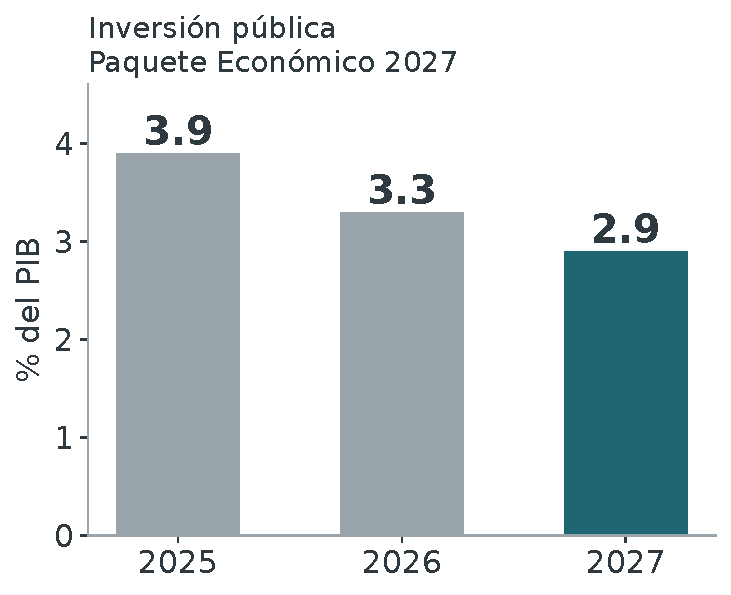
\includegraphics[height=0.62\textheight]{fig/l4_inversion_2027.pdf}
    \end{column}
  \end{columns}
  \fuente{Bolsa: actualización 2026, elaboración propia con datos de SHCP. Inversión: Paquete Económico 2027; fuente: CIEP (2026) con información de SHCP.}
\end{frame}

% ---------- 5. La deuda ya cuesta tanto como la Bolsa ----------
\begin{frame}{La deuda ya cuesta tanto como el margen de decisión}
  \centering
  \vspace{0.2em}
  \begin{tikzpicture}
    \node[draw=petroleo, line width=1.5pt, fill=fondo, rounded corners=4pt,
          minimum width=5.6cm, minimum height=3.4cm, align=center, text=gris] (b) {
      {\small Bolsa: margen de decisión}\\[0.3em]
      {\color{petroleo}\bfseries\fontsize{30}{34}\selectfont 4.0\,\%}\\[0.2em]
      {\small del PIB}\\[0.5em]
      {\footnotesize\color{grisclaro} Actualización 2026}};
    \node[draw=gris, line width=1.5pt, fill=white, rounded corners=4pt,
          minimum width=5.6cm, minimum height=3.4cm, align=center, text=gris,
          right=1.6cm of b] (d) {
      {\small Intereses de la deuda}\\[0.3em]
      {\color{gris}\bfseries\fontsize{30}{34}\selectfont 4.0\,\%}\\[0.2em]
      {\small del PIB}\\[0.5em]
      {\footnotesize\color{grisclaro} PPEF 2027 \;(3.8 en 2026)}};
    \node[font=\bfseries\fontsize{30}{34}\selectfont, text=petroleo] at ($(b.east)!0.5!(d.west)$) {=};
  \end{tikzpicture}\par
  \vspace{0.7em}
  {\large Por cada peso que queda para decidir, otro peso se va en intereses.\par}
  \fuente{\raggedright Bolsa y costo financiero 2026: actualización 2026, elaboración propia con datos de SHCP. Costo financiero 2027: PPEF 2027; fuente: CIEP con datos de SHCP. Razones con el PIB de SHCP; con un PIB más conservador serían algo mayores.\par}
\end{frame}

% ---------- 6. Lo que se aprobó para 2027 ----------
\begin{frame}{El paquete 2027 mueve la base en el margen; no cambia la restricción}
  \setbeamercolor{bloque}{bg=fondo,fg=gris}
  \begin{columns}[T]
    \begin{column}{0.48\textwidth}
      \frente{Amplía la base (en el margen)}{\punto Deducciones de ISR topadas en 96.67\,\% de los ingresos (empresas con ingresos >\,50\,mdp): impuesto mínimo de alrededor de 1\,\% de los ingresos.\par\vspace{0.5em}\punto Pérdidas fiscales: amortización hasta 50\,\% de la utilidad fiscal del ejercicio.}
    \end{column}
    \begin{column}{0.48\textwidth}
      \frente{Abarata el incumplimiento}{\punto Programa de regularización con condonación de 100\,\% de multas, recargos y gastos de ejecución.\par\vspace{0.5em}\punto Ampliado a grandes contribuyentes: se eliminó el tope de 300\,mdp de ingresos.}
    \end{column}
  \end{columns}
  \fuente{\raggedright Minutas aprobadas por la Cámara de Diputados en octubre de 2026. Fuente: minuta de reforma a la LISR; dictamen LIF 2027 (transitorio vigésimo primero) y reserva aprobada, Cámara de Diputados.\par}
\end{frame}

% ---------- 7. Una reforma pequeña no basta ----------
\begin{frame}{Una reforma pequeña no basta}
  \begin{columns}[c]
    \begin{column}{0.58\textwidth}
      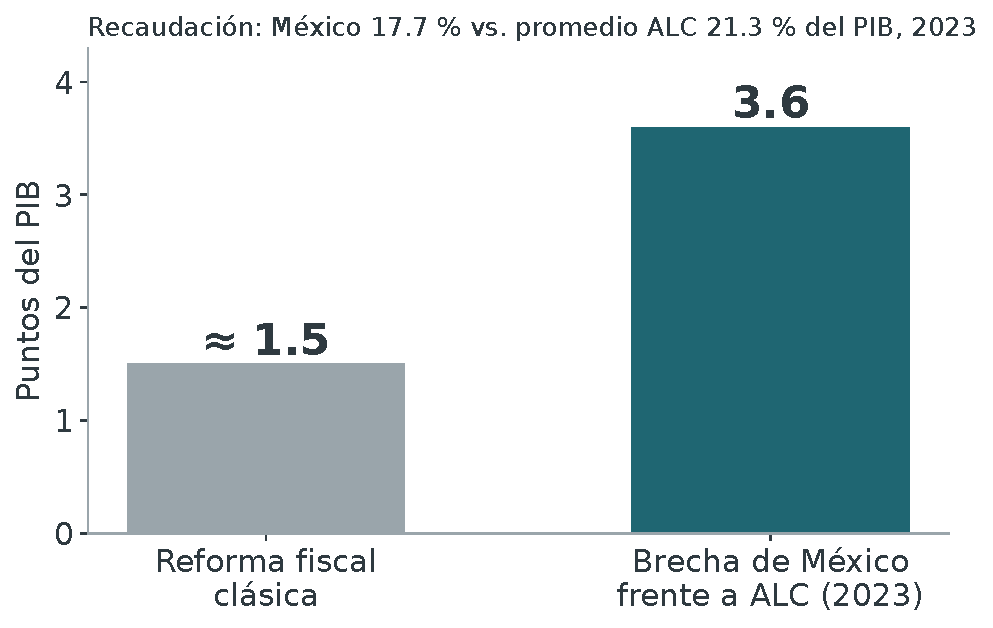
\includegraphics[width=\linewidth]{fig/l5_reforma_brecha.pdf}
    \end{column}
    \begin{column}{0.38\textwidth}
      \Large Una reforma fiscal clásica cubre
      {\color{petroleo}\bfseries menos de la mitad} de la brecha.
    \end{column}
  \end{columns}
  \fuente{Reforma clásica: del orden de 1.5 puntos del PIB. Brecha: OCDE, CEPAL, CIAT y BID (2026), \emph{Estadísticas tributarias en América Latina y el Caribe}, datos 2023, citado por CIEP (2026).}
\end{frame}

% ---------- 8. El tiempo juega en contra ----------
\begin{frame}{Sin reforma, la Bolsa se encoge cada año}
  \centering
  \begin{tikzpicture}[
      presion/.style={draw=grisclaro, line width=1pt, fill=white, rounded corners=3pt,
                      text width=4.1cm, minimum height=1.5cm, align=center, text=gris, font=\small,
                      execute at begin node={\hyphenpenalty=10000\relax}},
      flecha/.style={-{Stealth[length=3mm]}, line width=1.6pt, color=gris}]
    \node[draw=petroleo, line width=1.5pt, fill=fondo, rounded corners=4pt,
          minimum width=3.2cm, minimum height=1.9cm, align=center] (b)
          {{\color{petroleo}\bfseries\Large Bolsa}\\[0.1em]{\footnotesize margen de decisión}};
    \node[presion, left=0.7cm of b, yshift=0.9cm] (p1)
          {Pensiones contributivas de la generación de transición};
    \node[presion, left=0.7cm of b, yshift=-0.9cm] (p2)
          {Pensión no contributiva con rango constitucional};
    \node[presion, right=0.7cm of b] (p3)
          {Costo financiero\\de la deuda};
    \draw[flecha] (p1.east) -- (b.north west);
    \draw[flecha] (p2.east) -- (b.south west);
    \draw[flecha] (p3.west) -- (b.east);
  \end{tikzpicture}\par
  \vspace{1.2em}
  {\normalsize Ya ocurre: la inversión pública pasó de 3.9\,\% (2025) a 2.9\,\% del PIB (2027).\par}
  \fuente{Diagrama ilustrativo, sin escala. Inversión pública: Paquete Económico 2027; fuente: CIEP con datos de SHCP.}
\end{frame}

% ---------- 9. Cuatro frentes ----------
\begin{frame}{Cuatro frentes y una decisión}
  \vspace{-0.4em}
  \setbeamercolor{bloque}{bg=fondo,fg=gris}
  \begin{columns}[T]
    \begin{column}{0.48\textwidth}
      \frente{Reforma fiscal clásica (federal)}{Bases gravables, gastos fiscales, IVA, ISR.}\par\vspace{0.35em}
      \frente{Haciendas locales}{Ingresos propios de estados y municipios (predial, tenencia moderna) y financiamiento de sus funciones.}
    \end{column}
    \begin{column}{0.48\textwidth}
      \frente{Seguridad social}{Pensiones y salud con financiamiento sostenible e inclusión de trabajadores informales.}\par\vspace{0.35em}
      \frente{Empresas del Estado}{Pemex y CFE: reglas claras para los apoyos fiscales y registro transparente de los pasivos contingentes que hoy quedan fuera del presupuesto.}
    \end{column}
  \end{columns}
  \vfill
  \setbeamercolor{banda}{bg=petroleo,fg=white}
  \begin{beamercolorbox}[wd=\textwidth,sep=8pt,center]{banda}
    \bfseries Ninguno de los cuatro frentes cierra la cuenta por sí solo.\\
    Pensar a mediano plazo es decidir ahora el replanteamiento integral.
  \end{beamercolorbox}
  \vspace*{-0.6em}
\end{frame}

\end{document}
